% Options for packages loaded elsewhere
\PassOptionsToPackage{unicode}{hyperref}
\PassOptionsToPackage{hyphens}{url}
%
\documentclass[
]{article}
\usepackage{amsmath,amssymb}
\usepackage{iftex}
\ifPDFTeX
  \usepackage[T1]{fontenc}
  \usepackage[utf8]{inputenc}
  \usepackage{textcomp} % provide euro and other symbols
\else % if luatex or xetex
  \usepackage{unicode-math} % this also loads fontspec
  \defaultfontfeatures{Scale=MatchLowercase}
  \defaultfontfeatures[\rmfamily]{Ligatures=TeX,Scale=1}
\fi
\usepackage{lmodern}
\ifPDFTeX\else
  % xetex/luatex font selection
\fi
% Use upquote if available, for straight quotes in verbatim environments
\IfFileExists{upquote.sty}{\usepackage{upquote}}{}
\IfFileExists{microtype.sty}{% use microtype if available
  \usepackage[]{microtype}
  \UseMicrotypeSet[protrusion]{basicmath} % disable protrusion for tt fonts
}{}
\makeatletter
\@ifundefined{KOMAClassName}{% if non-KOMA class
  \IfFileExists{parskip.sty}{%
    \usepackage{parskip}
  }{% else
    \setlength{\parindent}{0pt}
    \setlength{\parskip}{6pt plus 2pt minus 1pt}}
}{% if KOMA class
  \KOMAoptions{parskip=half}}
\makeatother
\usepackage{xcolor}
\usepackage[margin=1in]{geometry}
\usepackage{color}
\usepackage{fancyvrb}
\newcommand{\VerbBar}{|}
\newcommand{\VERB}{\Verb[commandchars=\\\{\}]}
\DefineVerbatimEnvironment{Highlighting}{Verbatim}{commandchars=\\\{\}}
% Add ',fontsize=\small' for more characters per line
\usepackage{framed}
\definecolor{shadecolor}{RGB}{248,248,248}
\newenvironment{Shaded}{\begin{snugshade}}{\end{snugshade}}
\newcommand{\AlertTok}[1]{\textcolor[rgb]{0.94,0.16,0.16}{#1}}
\newcommand{\AnnotationTok}[1]{\textcolor[rgb]{0.56,0.35,0.01}{\textbf{\textit{#1}}}}
\newcommand{\AttributeTok}[1]{\textcolor[rgb]{0.13,0.29,0.53}{#1}}
\newcommand{\BaseNTok}[1]{\textcolor[rgb]{0.00,0.00,0.81}{#1}}
\newcommand{\BuiltInTok}[1]{#1}
\newcommand{\CharTok}[1]{\textcolor[rgb]{0.31,0.60,0.02}{#1}}
\newcommand{\CommentTok}[1]{\textcolor[rgb]{0.56,0.35,0.01}{\textit{#1}}}
\newcommand{\CommentVarTok}[1]{\textcolor[rgb]{0.56,0.35,0.01}{\textbf{\textit{#1}}}}
\newcommand{\ConstantTok}[1]{\textcolor[rgb]{0.56,0.35,0.01}{#1}}
\newcommand{\ControlFlowTok}[1]{\textcolor[rgb]{0.13,0.29,0.53}{\textbf{#1}}}
\newcommand{\DataTypeTok}[1]{\textcolor[rgb]{0.13,0.29,0.53}{#1}}
\newcommand{\DecValTok}[1]{\textcolor[rgb]{0.00,0.00,0.81}{#1}}
\newcommand{\DocumentationTok}[1]{\textcolor[rgb]{0.56,0.35,0.01}{\textbf{\textit{#1}}}}
\newcommand{\ErrorTok}[1]{\textcolor[rgb]{0.64,0.00,0.00}{\textbf{#1}}}
\newcommand{\ExtensionTok}[1]{#1}
\newcommand{\FloatTok}[1]{\textcolor[rgb]{0.00,0.00,0.81}{#1}}
\newcommand{\FunctionTok}[1]{\textcolor[rgb]{0.13,0.29,0.53}{\textbf{#1}}}
\newcommand{\ImportTok}[1]{#1}
\newcommand{\InformationTok}[1]{\textcolor[rgb]{0.56,0.35,0.01}{\textbf{\textit{#1}}}}
\newcommand{\KeywordTok}[1]{\textcolor[rgb]{0.13,0.29,0.53}{\textbf{#1}}}
\newcommand{\NormalTok}[1]{#1}
\newcommand{\OperatorTok}[1]{\textcolor[rgb]{0.81,0.36,0.00}{\textbf{#1}}}
\newcommand{\OtherTok}[1]{\textcolor[rgb]{0.56,0.35,0.01}{#1}}
\newcommand{\PreprocessorTok}[1]{\textcolor[rgb]{0.56,0.35,0.01}{\textit{#1}}}
\newcommand{\RegionMarkerTok}[1]{#1}
\newcommand{\SpecialCharTok}[1]{\textcolor[rgb]{0.81,0.36,0.00}{\textbf{#1}}}
\newcommand{\SpecialStringTok}[1]{\textcolor[rgb]{0.31,0.60,0.02}{#1}}
\newcommand{\StringTok}[1]{\textcolor[rgb]{0.31,0.60,0.02}{#1}}
\newcommand{\VariableTok}[1]{\textcolor[rgb]{0.00,0.00,0.00}{#1}}
\newcommand{\VerbatimStringTok}[1]{\textcolor[rgb]{0.31,0.60,0.02}{#1}}
\newcommand{\WarningTok}[1]{\textcolor[rgb]{0.56,0.35,0.01}{\textbf{\textit{#1}}}}
\usepackage{graphicx}
\makeatletter
\def\maxwidth{\ifdim\Gin@nat@width>\linewidth\linewidth\else\Gin@nat@width\fi}
\def\maxheight{\ifdim\Gin@nat@height>\textheight\textheight\else\Gin@nat@height\fi}
\makeatother
% Scale images if necessary, so that they will not overflow the page
% margins by default, and it is still possible to overwrite the defaults
% using explicit options in \includegraphics[width, height, ...]{}
\setkeys{Gin}{width=\maxwidth,height=\maxheight,keepaspectratio}
% Set default figure placement to htbp
\makeatletter
\def\fps@figure{htbp}
\makeatother
\setlength{\emergencystretch}{3em} % prevent overfull lines
\providecommand{\tightlist}{%
  \setlength{\itemsep}{0pt}\setlength{\parskip}{0pt}}
\setcounter{secnumdepth}{-\maxdimen} % remove section numbering
\newlength{\cslhangindent}
\setlength{\cslhangindent}{1.5em}
\newlength{\csllabelwidth}
\setlength{\csllabelwidth}{3em}
\newlength{\cslentryspacingunit} % times entry-spacing
\setlength{\cslentryspacingunit}{\parskip}
\newenvironment{CSLReferences}[2] % #1 hanging-ident, #2 entry spacing
 {% don't indent paragraphs
  \setlength{\parindent}{0pt}
  % turn on hanging indent if param 1 is 1
  \ifodd #1
  \let\oldpar\par
  \def\par{\hangindent=\cslhangindent\oldpar}
  \fi
  % set entry spacing
  \setlength{\parskip}{#2\cslentryspacingunit}
 }%
 {}
\usepackage{calc}
\newcommand{\CSLBlock}[1]{#1\hfill\break}
\newcommand{\CSLLeftMargin}[1]{\parbox[t]{\csllabelwidth}{#1}}
\newcommand{\CSLRightInline}[1]{\parbox[t]{\linewidth - \csllabelwidth}{#1}\break}
\newcommand{\CSLIndent}[1]{\hspace{\cslhangindent}#1}
\ifLuaTeX
  \usepackage{selnolig}  % disable illegal ligatures
\fi
\IfFileExists{bookmark.sty}{\usepackage{bookmark}}{\usepackage{hyperref}}
\IfFileExists{xurl.sty}{\usepackage{xurl}}{} % add URL line breaks if available
\urlstyle{same}
\hypersetup{
  pdftitle={Exercise: Two-way ANOVA in R},
  pdfauthor={Stephan Huber},
  hidelinks,
  pdfcreator={LaTeX via pandoc}}

\title{Exercise: Two-way ANOVA in R}
\author{Stephan Huber}
\date{2024-01-16}

\begin{document}
\maketitle
\begin{abstract}
This is an exercise where data management with the \texttt{dplyr}
functions \texttt{pivot\_longer}, \texttt{rename}, and
\texttt{bind\_rows} is practiced. Moreover, I exemplify how an ANOVA
analysis can be executed with R. Doing so I refer to the content of
Childs et al. (2021, Chapter 27). All data to this exercise can be found
in Huber (2024).
\end{abstract}

\hypertarget{read}{%
\section{Read}\label{read}}

Read Childs et al. (2021):
\href{https://dzchilds.github.io/stats-for-bio/two-way-anova-in-r.html}{27.2
Competition between Calluna and Festuca}.

Our goal is to learn how to work with two-way ANOVA models in R, using
an example from a plant competition experiment. The work flow is very
similar to one-way ANOVA in R. We'll start with the problem and the
data, and then work through model fitting, evaluating assumptions,
significance testing, and finally, presenting the results.

\hypertarget{set-up-the-r-session}{%
\section{Set up the R session}\label{set-up-the-r-session}}

Download and open the script that you find
\href{https://raw.githubusercontent.com/hubchev/ewa/main/rmd_festuca/r_festuca.R}{here}.
This script contains all the code that is shown below. The solutions to
the exercises can be found
\href{https://raw.githubusercontent.com/hubchev/ewa/main/rmd_festuca/r_festuca_solutions.R}{here}.

\begin{Shaded}
\begin{Highlighting}[]
\CommentTok{\# setwd("\textasciitilde{}/Dropbox/hsf/courses/ewa/ewa\_all")}

\FunctionTok{rm}\NormalTok{(}\AttributeTok{list =} \FunctionTok{ls}\NormalTok{())}

\ControlFlowTok{if}\NormalTok{ (}\SpecialCharTok{!}\FunctionTok{require}\NormalTok{(pacman)) }\FunctionTok{install.packages}\NormalTok{(}\StringTok{"pacman"}\NormalTok{)}
\end{Highlighting}
\end{Shaded}

\begin{verbatim}
## Loading required package: pacman
\end{verbatim}

\begin{Shaded}
\begin{Highlighting}[]
\NormalTok{pacman}\SpecialCharTok{::}\FunctionTok{p\_load}\NormalTok{(tidyverse, rstatix, ggpubr, agricolae)}
\end{Highlighting}
\end{Shaded}

\hypertarget{create-a-data-frame}{%
\section{Create a data frame}\label{create-a-data-frame}}

Plants have an optimal soil pH for growth, and this varies between
species. Consequently we would expect that if we grow two plants in
competition with each other at different pH values the effect of
competition might vary according to the soil pH. In a recent study the
growth of the grass Festuca ovina (Sheep's Fescue) in competition with
the heather Calluna vulgaris (Ling) was investigated in soils with
different pH. Calluna is well adapted to grow on very acidic soils such
as on the Millstone grit and blanket bogs around Sheffield. Festuca
grows on soils with a much wider range of pH. We might hypothesise that
Calluna will be a better competitor of Festuca in very acid soils than
in moderately acid soils. Here are the data: The column (Weight)
contains the Festuca dry weights, (pH) contains the codes for the pH
treatment (levels: pH3.5, pH5.5), the column (Calluna) contains the
codes for the presence or absence of Calluna (levels: Present, Absent).

\begin{Shaded}
\begin{Highlighting}[]
\NormalTok{data\_present }\OtherTok{\textless{}{-}} \FunctionTok{data.frame}\NormalTok{(}
  \AttributeTok{Condition =} \FunctionTok{rep}\NormalTok{(}\FunctionTok{c}\NormalTok{(}\StringTok{"Calluna Present"}\NormalTok{), }\AttributeTok{each =} \DecValTok{5}\NormalTok{),}
  \StringTok{\textasciigrave{}}\AttributeTok{pH 3.5}\StringTok{\textasciigrave{}} \OtherTok{=} \FunctionTok{c}\NormalTok{(}\FloatTok{2.76}\NormalTok{, }\FloatTok{2.39}\NormalTok{, }\FloatTok{3.54}\NormalTok{, }\FloatTok{3.71}\NormalTok{, }\FloatTok{2.49}\NormalTok{),}
  \StringTok{\textasciigrave{}}\AttributeTok{pH 5.5}\StringTok{\textasciigrave{}} \OtherTok{=} \FunctionTok{c}\NormalTok{(}\FloatTok{3.21}\NormalTok{, }\FloatTok{4.10}\NormalTok{, }\FloatTok{3.04}\NormalTok{, }\FloatTok{4.13}\NormalTok{, }\FloatTok{5.21}\NormalTok{),}
  \AttributeTok{check.names =} \ConstantTok{FALSE}
\NormalTok{)}
\NormalTok{data\_present}
\end{Highlighting}
\end{Shaded}

\begin{verbatim}
##         Condition pH 3.5 pH 5.5
## 1 Calluna Present   2.76   3.21
## 2 Calluna Present   2.39   4.10
## 3 Calluna Present   3.54   3.04
## 4 Calluna Present   3.71   4.13
## 5 Calluna Present   2.49   5.21
\end{verbatim}

\begin{Shaded}
\begin{Highlighting}[]
\NormalTok{data\_absent }\OtherTok{\textless{}{-}} \FunctionTok{data.frame}\NormalTok{(}
  \AttributeTok{Condition =} \FunctionTok{rep}\NormalTok{(}\FunctionTok{c}\NormalTok{(}\StringTok{"Calluna Absent"}\NormalTok{), }\AttributeTok{each =} \DecValTok{5}\NormalTok{),}
  \StringTok{\textasciigrave{}}\AttributeTok{pH 3.5}\StringTok{\textasciigrave{}} \OtherTok{=} \FunctionTok{c}\NormalTok{(}\FloatTok{4.10}\NormalTok{, }\FloatTok{2.72}\NormalTok{, }\FloatTok{2.28}\NormalTok{, }\FloatTok{4.43}\NormalTok{, }\FloatTok{3.31}\NormalTok{),}
  \StringTok{\textasciigrave{}}\AttributeTok{pH 5.5}\StringTok{\textasciigrave{}} \OtherTok{=} \FunctionTok{c}\NormalTok{(}\FloatTok{5.92}\NormalTok{, }\FloatTok{7.31}\NormalTok{, }\FloatTok{6.10}\NormalTok{, }\FloatTok{5.25}\NormalTok{, }\FloatTok{7.45}\NormalTok{),}
  \AttributeTok{check.names =} \ConstantTok{FALSE}
\NormalTok{)}
\NormalTok{data\_absent}
\end{Highlighting}
\end{Shaded}

\begin{verbatim}
##        Condition pH 3.5 pH 5.5
## 1 Calluna Absent   4.10   5.92
## 2 Calluna Absent   2.72   7.31
## 3 Calluna Absent   2.28   6.10
## 4 Calluna Absent   4.43   5.25
## 5 Calluna Absent   3.31   7.45
\end{verbatim}

\hypertarget{make-the-data-long}{%
\section{Make the data ``long''}\label{make-the-data-long}}

Read the \href{https://dplyr.tidyverse.org/reference/bind_rows.html}{R
documentation} of the function \texttt{bind\_rows} which is part of the
\texttt{dplyr} package.

Combine the objects \texttt{data\_present} and \texttt{data\_absent}.

\begin{verbatim}
##          Condition pH 3.5 pH 5.5
## 1  Calluna Present   2.76   3.21
## 2  Calluna Present   2.39   4.10
## 3  Calluna Present   3.54   3.04
## 4  Calluna Present   3.71   4.13
## 5  Calluna Present   2.49   5.21
## 6   Calluna Absent   4.10   5.92
## 7   Calluna Absent   2.72   7.31
## 8   Calluna Absent   2.28   6.10
## 9   Calluna Absent   4.43   5.25
## 10  Calluna Absent   3.31   7.45
\end{verbatim}

Read Wickham \& Grolemund (2023):
\href{https://r4ds.hadley.nz/data-tidy\#sec-pivoting}{5.3 Lengthening
data}.

Rearrange the data so that they look like this:

\begin{Shaded}
\begin{Highlighting}[]
\NormalTok{festuca}
\end{Highlighting}
\end{Shaded}

\begin{verbatim}
## # A tibble: 20 x 3
##    Calluna         pH     Weight
##    <chr>           <chr>   <dbl>
##  1 Calluna Present pH 3.5   2.76
##  2 Calluna Present pH 5.5   3.21
##  3 Calluna Present pH 3.5   2.39
##  4 Calluna Present pH 5.5   4.1 
##  5 Calluna Present pH 3.5   3.54
##  6 Calluna Present pH 5.5   3.04
##  7 Calluna Present pH 3.5   3.71
##  8 Calluna Present pH 5.5   4.13
##  9 Calluna Present pH 3.5   2.49
## 10 Calluna Present pH 5.5   5.21
## 11 Calluna Absent  pH 3.5   4.1 
## 12 Calluna Absent  pH 5.5   5.92
## 13 Calluna Absent  pH 3.5   2.72
## 14 Calluna Absent  pH 5.5   7.31
## 15 Calluna Absent  pH 3.5   2.28
## 16 Calluna Absent  pH 5.5   6.1 
## 17 Calluna Absent  pH 3.5   4.43
## 18 Calluna Absent  pH 5.5   5.25
## 19 Calluna Absent  pH 3.5   3.31
## 20 Calluna Absent  pH 5.5   7.45
\end{verbatim}

\hypertarget{descriptive-statistics}{%
\section{Descriptive Statistics}\label{descriptive-statistics}}

Calculate the following statistics and graphs:

\begin{Shaded}
\begin{Highlighting}[]
\NormalTok{summary\_stats}
\end{Highlighting}
\end{Shaded}

\begin{verbatim}
## # A tibble: 4 x 4
##   Calluna         pH      mean   var
##   <chr>           <chr>  <dbl> <dbl>
## 1 Calluna Absent  pH 3.5  3.37 0.818
## 2 Calluna Absent  pH 5.5  6.41 0.893
## 3 Calluna Present pH 3.5  2.98 0.371
## 4 Calluna Present pH 5.5  3.94 0.754
\end{verbatim}

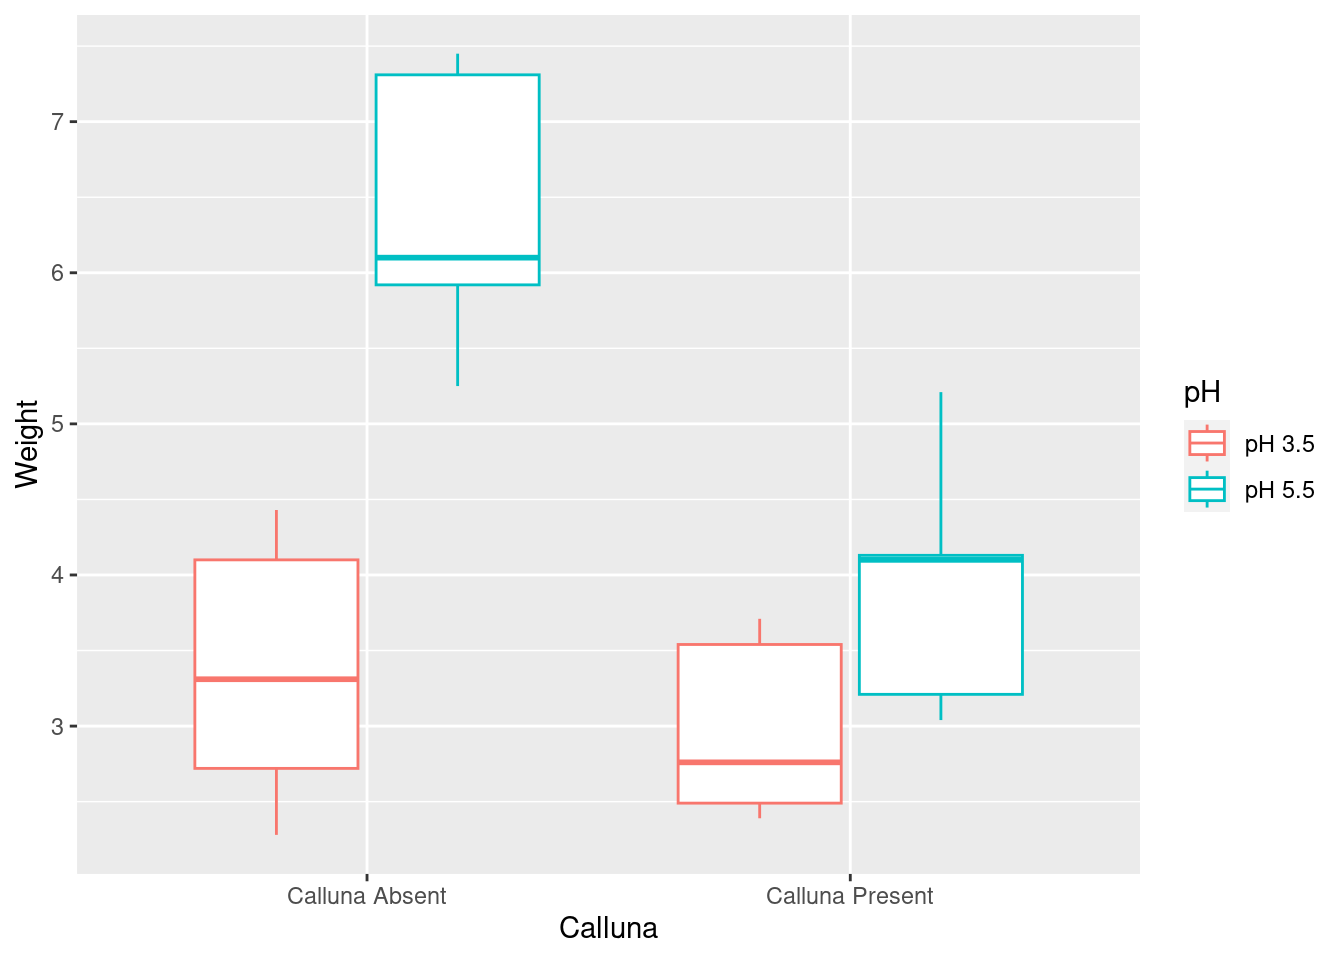
\includegraphics{rmd_festuca_files/figure-latex/unnamed-chunk-8-1.pdf}

\hypertarget{anova}{%
\section{ANOVA}\label{anova}}

Use this model to calculate the ANOVA:
\texttt{Weight\ \textasciitilde{}\ pH\ +\ Calluna\ +\ pH:Calluna}

\begin{verbatim}
## Analysis of Variance Table
## 
## Response: Weight
##            Df  Sum Sq Mean Sq F value    Pr(>F)    
## pH          1 19.9800 19.9800 28.1792 7.065e-05 ***
## Calluna     1 10.2102 10.2102 14.4001   0.00159 ** 
## pH:Calluna  1  5.3976  5.3976  7.6126   0.01397 *  
## Residuals  16 11.3446  0.7090                      
## ---
## Signif. codes:  0 '***' 0.001 '**' 0.01 '*' 0.05 '.' 0.1 ' ' 1
\end{verbatim}

\hypertarget{diagnostics}{%
\section{Diagnostics}\label{diagnostics}}

Read Childs et al. (2021):
\href{https://dzchilds.github.io/stats-for-bio/two-way-anova-in-r.html\#diagnostics}{27.5
Diagnostics}. Moreover,
\href{https://www.datanovia.com/en/lessons/anova-in-r/}{this page} is
worth a look. You find some alternatives R functions that you may find
helpful for ANOVA diagnostics.

\begin{Shaded}
\begin{Highlighting}[]
\FunctionTok{plot}\NormalTok{(festuca\_model, }\AttributeTok{which =} \DecValTok{2}\NormalTok{, }\AttributeTok{add.smooth =} \ConstantTok{FALSE}\NormalTok{)}
\end{Highlighting}
\end{Shaded}

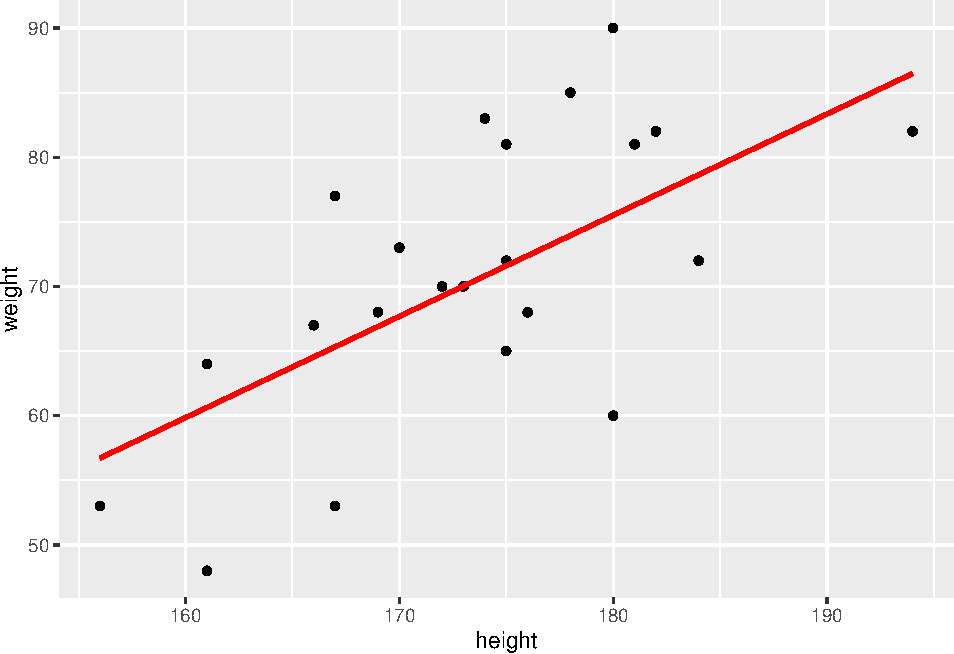
\includegraphics{rmd_festuca_files/figure-latex/unnamed-chunk-11-1.pdf}

\begin{Shaded}
\begin{Highlighting}[]
\FunctionTok{plot}\NormalTok{(festuca\_model, }\AttributeTok{which =} \DecValTok{3}\NormalTok{, }\AttributeTok{add.smooth =} \ConstantTok{FALSE}\NormalTok{)}
\end{Highlighting}
\end{Shaded}

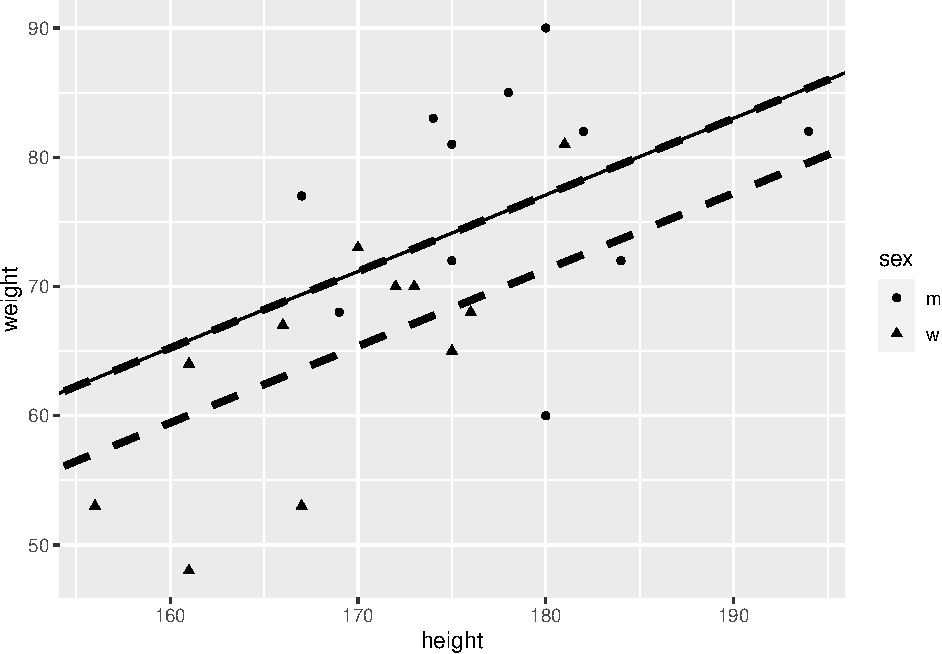
\includegraphics{rmd_festuca_files/figure-latex/unnamed-chunk-12-1.pdf}

\hypertarget{interaction-diagram}{%
\section{Interaction Diagram}\label{interaction-diagram}}

Can you use the function \texttt{interaction.plot} to create the
following:
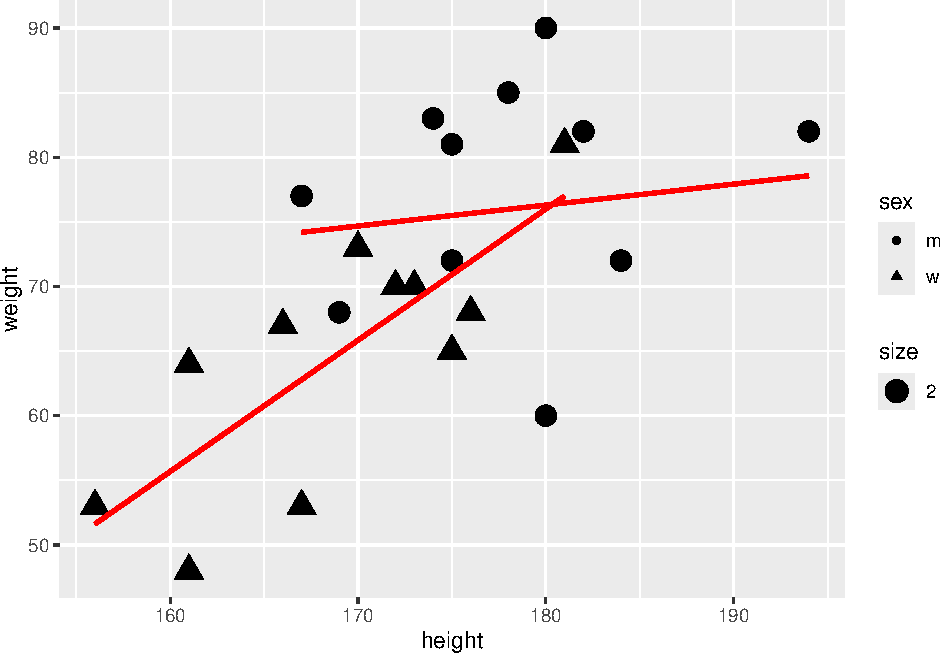
\includegraphics{rmd_festuca_files/figure-latex/unnamed-chunk-13-1.pdf}

Here is a much nicer and more flexible approach to make interaction
plots using \texttt{tidyverse} functions:

\begin{Shaded}
\begin{Highlighting}[]
\CommentTok{\# step 1. calculate means for each treatment combination}
\NormalTok{festuca\_means }\OtherTok{\textless{}{-}} 
\NormalTok{  festuca }\SpecialCharTok{\%\textgreater{}\%} 
  \FunctionTok{group\_by}\NormalTok{(Calluna, pH) }\SpecialCharTok{\%\textgreater{}\%} \CommentTok{\# \textless{}{-} remember to group by *both* factors}
  \FunctionTok{summarise}\NormalTok{(}\AttributeTok{Means =} \FunctionTok{mean}\NormalTok{(Weight))}
\end{Highlighting}
\end{Shaded}

\begin{Shaded}
\begin{Highlighting}[]
\CommentTok{\# step 2. plot these as an interaction plot}
\FunctionTok{ggplot}\NormalTok{(festuca\_means, }
       \FunctionTok{aes}\NormalTok{(}\AttributeTok{x =}\NormalTok{ Calluna, }\AttributeTok{y =}\NormalTok{ Means, }\AttributeTok{colour =}\NormalTok{ pH, }\AttributeTok{group =}\NormalTok{ pH)) }\SpecialCharTok{+}
  \FunctionTok{geom\_point}\NormalTok{(}\AttributeTok{size =} \DecValTok{4}\NormalTok{) }\SpecialCharTok{+} \FunctionTok{geom\_line}\NormalTok{()}
\end{Highlighting}
\end{Shaded}

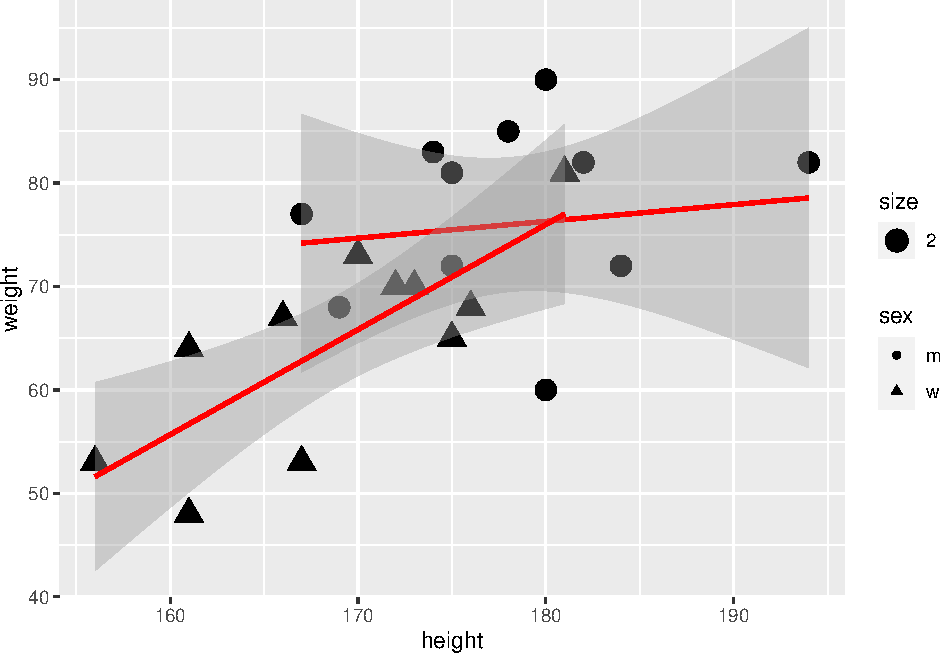
\includegraphics{rmd_festuca_files/figure-latex/unnamed-chunk-15-1.pdf}

Read Childs et al. (2021):
\href{https://dzchilds.github.io/stats-for-bio/two-way-anova-in-r.html\#understanding-the-model-graphically}{27.6.1}
and consider the following figure:

\includegraphics{https://dzchilds.github.io/stats-for-bio/images/interaction-diagrams.png}

\hypertarget{multiple-comparison-tests}{%
\section{Multiple comparison tests}\label{multiple-comparison-tests}}

\begin{Shaded}
\begin{Highlighting}[]
\FunctionTok{TukeyHSD}\NormalTok{(festuca\_model, }\AttributeTok{which =} \StringTok{\textquotesingle{}pH:Calluna\textquotesingle{}}\NormalTok{)}
\end{Highlighting}
\end{Shaded}

\begin{verbatim}
##   Tukey multiple comparisons of means
##     95% family-wise confidence level
## 
## Fit: aov(formula = Weight ~ pH + Calluna + pH:Calluna, data = festuca)
## 
## $`pH:Calluna`
##                                                 diff        lwr        upr
## pH 5.5:Calluna Absent-pH 3.5:Calluna Absent    3.038  1.5143518  4.5616482
## pH 3.5:Calluna Present-pH 3.5:Calluna Absent  -0.390 -1.9136482  1.1336482
## pH 5.5:Calluna Present-pH 3.5:Calluna Absent   0.570 -0.9536482  2.0936482
## pH 3.5:Calluna Present-pH 5.5:Calluna Absent  -3.428 -4.9516482 -1.9043518
## pH 5.5:Calluna Present-pH 5.5:Calluna Absent  -2.468 -3.9916482 -0.9443518
## pH 5.5:Calluna Present-pH 3.5:Calluna Present  0.960 -0.5636482  2.4836482
##                                                   p adj
## pH 5.5:Calluna Absent-pH 3.5:Calluna Absent   0.0001731
## pH 3.5:Calluna Present-pH 3.5:Calluna Absent  0.8826936
## pH 5.5:Calluna Present-pH 3.5:Calluna Absent  0.7117913
## pH 3.5:Calluna Present-pH 5.5:Calluna Absent  0.0000443
## pH 5.5:Calluna Present-pH 5.5:Calluna Absent  0.0014155
## pH 5.5:Calluna Present-pH 3.5:Calluna Present 0.3079685
\end{verbatim}

\begin{verbatim}


```r
HSD.test(festuca_model, trt = c("pH", "Calluna"), console = TRUE)
\end{verbatim}

\begin{verbatim}
## 
## Study: festuca_model ~ c("pH", "Calluna")
## 
## HSD Test for Weight 
## 
## Mean Square Error:  0.709035 
## 
## pH:Calluna,  means
## 
##                        Weight       std r        se  Min  Max  Q25  Q50  Q75
## pH 3.5:Calluna Absent   3.368 0.9042511 5 0.3765727 2.28 4.43 2.72 3.31 4.10
## pH 3.5:Calluna Present  2.978 0.6089089 5 0.3765727 2.39 3.71 2.49 2.76 3.54
## pH 5.5:Calluna Absent   6.406 0.9451614 5 0.3765727 5.25 7.45 5.92 6.10 7.31
## pH 5.5:Calluna Present  3.938 0.8685448 5 0.3765727 3.04 5.21 3.21 4.10 4.13
## 
## Alpha: 0.05 ; DF Error: 16 
## Critical Value of Studentized Range: 4.046093 
## 
## Minimun Significant Difference: 1.523648 
## 
## Treatments with the same letter are not significantly different.
## 
##                        Weight groups
## pH 5.5:Calluna Absent   6.406      a
## pH 5.5:Calluna Present  3.938      b
## pH 3.5:Calluna Absent   3.368      b
## pH 3.5:Calluna Present  2.978      b
\end{verbatim}

\hypertarget{drawing-conclusions-and-presenting-results}{%
\section{Drawing conclusions and presenting
results}\label{drawing-conclusions-and-presenting-results}}

Here are some code examples how the shown graphs above could be made
much nicer.

\begin{Shaded}
\begin{Highlighting}[]
\CommentTok{\# step 1. calculate means for each treatment combination}
\NormalTok{festuca\_stats }\OtherTok{\textless{}{-}} 
\NormalTok{  festuca }\SpecialCharTok{\%\textgreater{}\%} 
  \FunctionTok{group\_by}\NormalTok{(Calluna, pH) }\SpecialCharTok{\%\textgreater{}\%} \CommentTok{\# \textless{}{-} remember to group by the two factors}
  \FunctionTok{summarise}\NormalTok{(}\AttributeTok{Means =} \FunctionTok{mean}\NormalTok{(Weight), }\AttributeTok{SEs =} \FunctionTok{sd}\NormalTok{(Weight)}\SpecialCharTok{/}\FunctionTok{sqrt}\NormalTok{(}\FunctionTok{n}\NormalTok{()))}
\end{Highlighting}
\end{Shaded}

\begin{verbatim}
## `summarise()` has grouped output by 'Calluna'. You can override using the
## `.groups` argument.
\end{verbatim}

\begin{Shaded}
\begin{Highlighting}[]
\CommentTok{\# step 1. calculate means for each treatment combination}
\NormalTok{festuca\_stats }\OtherTok{\textless{}{-}} 
\NormalTok{  festuca }\SpecialCharTok{\%\textgreater{}\%} 
  \FunctionTok{group\_by}\NormalTok{(Calluna, pH) }\SpecialCharTok{\%\textgreater{}\%} \CommentTok{\# \textless{}{-} remember to group by the two factors}
  \FunctionTok{summarise}\NormalTok{(}\AttributeTok{Means =} \FunctionTok{mean}\NormalTok{(Weight), }\AttributeTok{SEs =} \FunctionTok{sd}\NormalTok{(Weight)}\SpecialCharTok{/}\FunctionTok{sqrt}\NormalTok{(}\FunctionTok{n}\NormalTok{()))}
\end{Highlighting}
\end{Shaded}

\begin{Shaded}
\begin{Highlighting}[]
\CommentTok{\# step 2. plot these as an interaction plot}
\FunctionTok{ggplot}\NormalTok{(festuca\_stats, }
       \FunctionTok{aes}\NormalTok{(}\AttributeTok{x =}\NormalTok{ Calluna, }\AttributeTok{y =}\NormalTok{ Means, }\AttributeTok{colour =}\NormalTok{ pH,}
           \AttributeTok{ymin =}\NormalTok{ Means }\SpecialCharTok{{-}}\NormalTok{ SEs, }\AttributeTok{ymax =}\NormalTok{ Means }\SpecialCharTok{+}\NormalTok{ SEs)) }\SpecialCharTok{+}
  \CommentTok{\# this adds the mean}
  \FunctionTok{geom\_point}\NormalTok{(}\AttributeTok{size =} \DecValTok{3}\NormalTok{) }\SpecialCharTok{+}
  \CommentTok{\# this adds the error bars}
  \FunctionTok{geom\_errorbar}\NormalTok{(}\AttributeTok{width =} \FloatTok{0.1}\NormalTok{) }\SpecialCharTok{+}
  \CommentTok{\# controlling the appearance}
  \FunctionTok{scale\_y\_continuous}\NormalTok{(}\AttributeTok{limits =} \FunctionTok{c}\NormalTok{(}\DecValTok{2}\NormalTok{, }\DecValTok{7}\NormalTok{)) }\SpecialCharTok{+} 
  \FunctionTok{xlab}\NormalTok{(}\StringTok{"Calluna"}\NormalTok{) }\SpecialCharTok{+} \FunctionTok{ylab}\NormalTok{(}\StringTok{"Festuca yield (g dry weight)"}\NormalTok{) }\SpecialCharTok{+} 
  \CommentTok{\# use a more professional theme}
  \FunctionTok{theme\_bw}\NormalTok{()}
\end{Highlighting}
\end{Shaded}

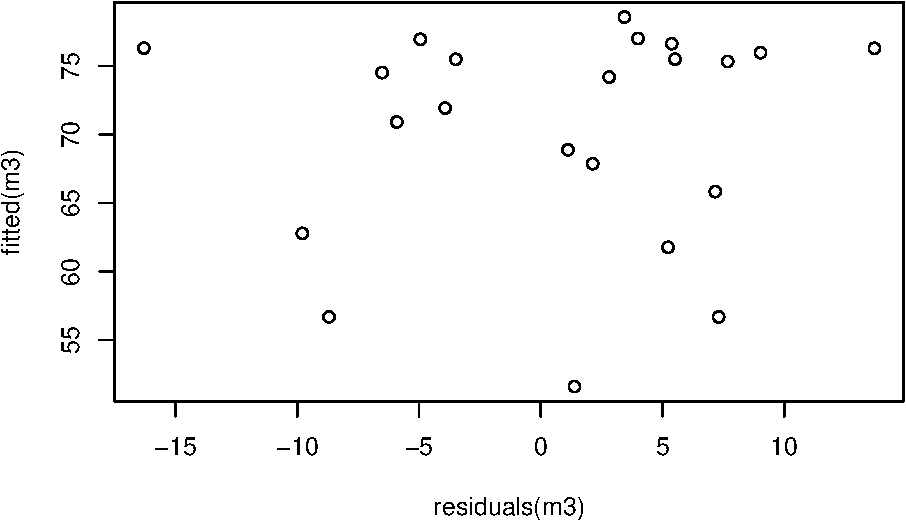
\includegraphics{rmd_festuca_files/figure-latex/unnamed-chunk-20-1.pdf}

\begin{Shaded}
\begin{Highlighting}[]
\CommentTok{\# define a position adjustment }
\NormalTok{pos }\OtherTok{\textless{}{-}} \FunctionTok{position\_dodge}\NormalTok{(}\FloatTok{0.15}\NormalTok{)}
\CommentTok{\# make the plot}
\FunctionTok{ggplot}\NormalTok{(festuca\_stats, }
       \FunctionTok{aes}\NormalTok{(}\AttributeTok{x =}\NormalTok{ Calluna, }\AttributeTok{y =}\NormalTok{ Means, }\AttributeTok{colour =}\NormalTok{ pH,}
           \AttributeTok{ymin =}\NormalTok{ Means }\SpecialCharTok{{-}}\NormalTok{ SEs, }\AttributeTok{ymax =}\NormalTok{ Means }\SpecialCharTok{+}\NormalTok{ SEs)) }\SpecialCharTok{+}
  \CommentTok{\# this adds the mean (shift positions with \textquotesingle{}position =\textquotesingle{})}
  \FunctionTok{geom\_point}\NormalTok{(}\AttributeTok{size =} \DecValTok{3}\NormalTok{, }\AttributeTok{position =}\NormalTok{ pos) }\SpecialCharTok{+}
  \CommentTok{\# this adds the error bars (shift positions with \textquotesingle{}position =\textquotesingle{})}
  \FunctionTok{geom\_errorbar}\NormalTok{(}\AttributeTok{width =} \FloatTok{0.1}\NormalTok{, }\AttributeTok{position =}\NormalTok{ pos) }\SpecialCharTok{+}
  \CommentTok{\# controlling the appearance}
  \FunctionTok{scale\_y\_continuous}\NormalTok{(}\AttributeTok{limits =} \FunctionTok{c}\NormalTok{(}\DecValTok{2}\NormalTok{, }\DecValTok{7}\NormalTok{)) }\SpecialCharTok{+} 
  \FunctionTok{xlab}\NormalTok{(}\StringTok{"Calluna"}\NormalTok{) }\SpecialCharTok{+} \FunctionTok{ylab}\NormalTok{(}\StringTok{"Festuca yield (g dry weight)"}\NormalTok{) }\SpecialCharTok{+} 
  \CommentTok{\# use a more professional theme}
  \FunctionTok{theme\_bw}\NormalTok{()}
\end{Highlighting}
\end{Shaded}

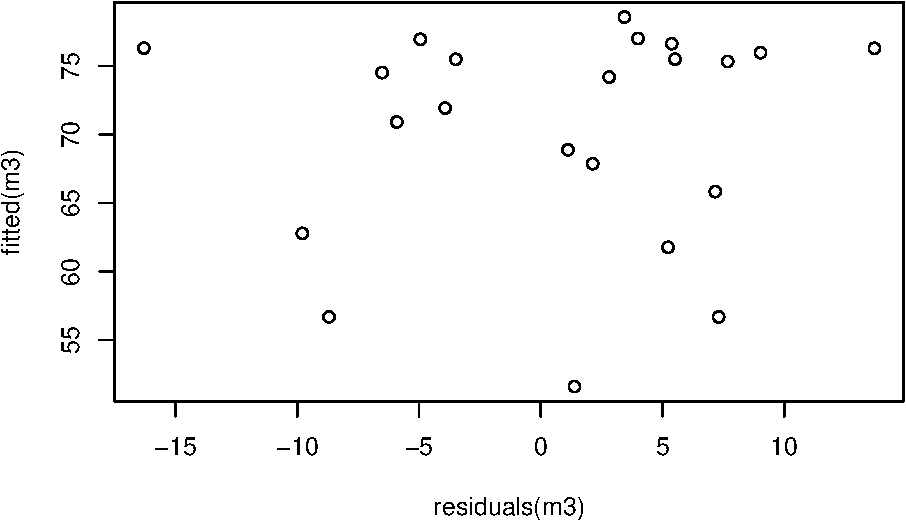
\includegraphics{rmd_festuca_files/figure-latex/unnamed-chunk-21-1.pdf}

\begin{Shaded}
\begin{Highlighting}[]
\FunctionTok{ggplot}\NormalTok{(festuca\_stats, }
       \FunctionTok{aes}\NormalTok{(}\AttributeTok{x =}\NormalTok{ Calluna, }\AttributeTok{y =}\NormalTok{ Means, }\AttributeTok{fill =}\NormalTok{ pH,}
           \AttributeTok{ymin =}\NormalTok{ Means }\SpecialCharTok{{-}}\NormalTok{ SEs, }\AttributeTok{ymax =}\NormalTok{ Means }\SpecialCharTok{+}\NormalTok{ SEs)) }\SpecialCharTok{+}
  \CommentTok{\# this adds the mean}
  \FunctionTok{geom\_col}\NormalTok{(}\AttributeTok{position =} \FunctionTok{position\_dodge}\NormalTok{()) }\SpecialCharTok{+}
  \CommentTok{\# this adds the error bars}
  \FunctionTok{geom\_errorbar}\NormalTok{(}\AttributeTok{position =} \FunctionTok{position\_dodge}\NormalTok{(}\FloatTok{0.9}\NormalTok{), }\AttributeTok{width=}\NormalTok{.}\DecValTok{2}\NormalTok{) }\SpecialCharTok{+}
  \CommentTok{\# controlling the appearance}
  \FunctionTok{xlab}\NormalTok{(}\StringTok{"Calluna"}\NormalTok{) }\SpecialCharTok{+} \FunctionTok{ylab}\NormalTok{(}\StringTok{"Festuca yield (g dry weight)"}\NormalTok{)}
\end{Highlighting}
\end{Shaded}

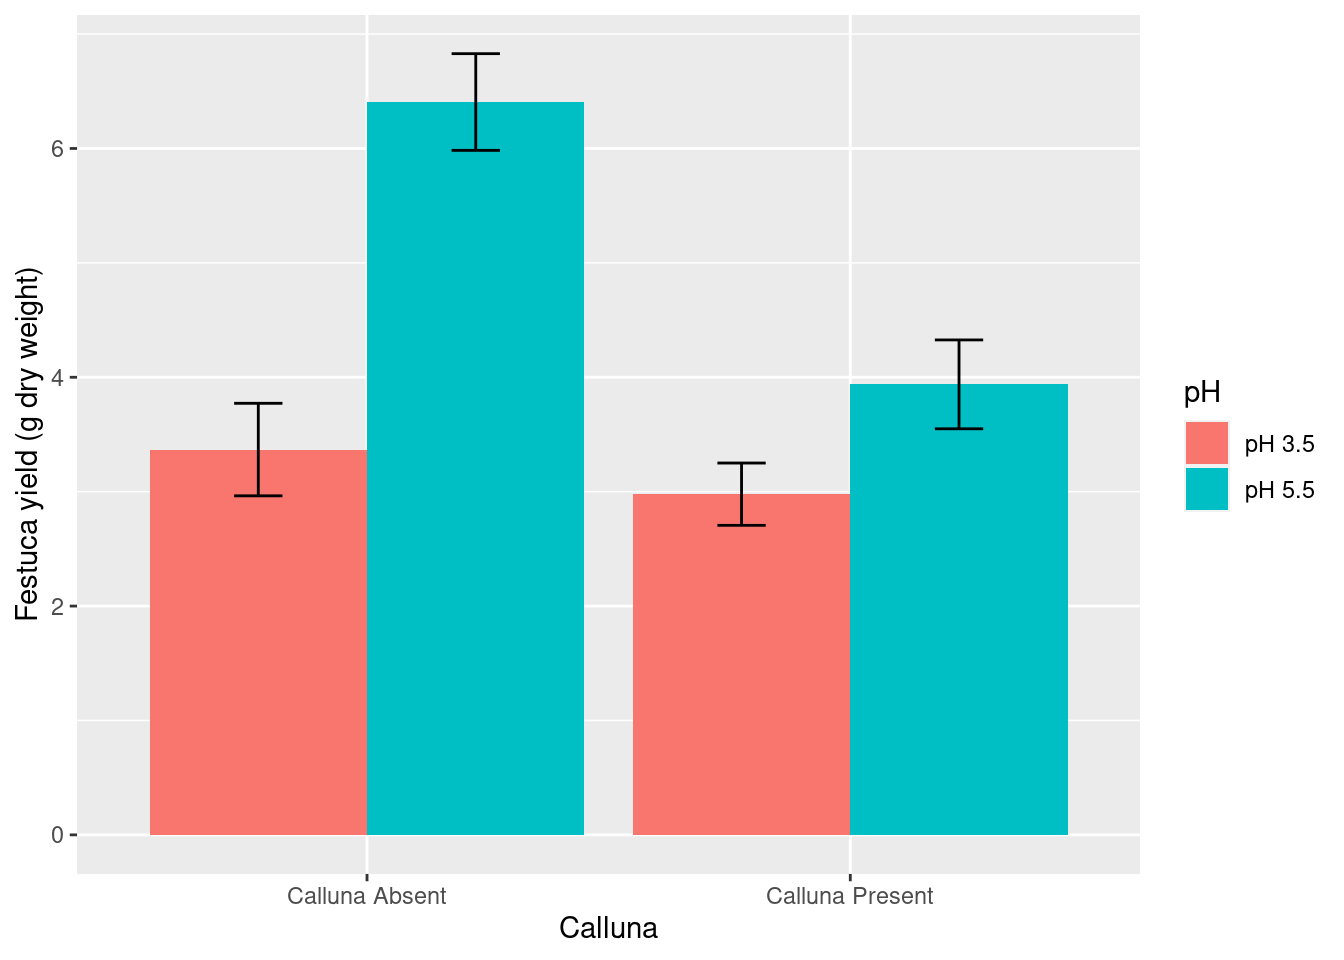
\includegraphics{rmd_festuca_files/figure-latex/unnamed-chunk-22-1.pdf}

\hypertarget{references}{%
\section*{References}\label{references}}
\addcontentsline{toc}{section}{References}

\hypertarget{refs}{}
\begin{CSLReferences}{1}{0}
\leavevmode\vadjust pre{\hypertarget{ref-Childs2021APS}{}}%
Childs, D. Z., Hindle, B. J., \& Warren, P. H. (2021). \emph{APS 240:
Data analysis and statistics with r}. online.
\url{https://dzchilds.github.io/stats-for-bio}

\leavevmode\vadjust pre{\hypertarget{ref-Huber2024Empirisch}{}}%
Huber, S. (2024). \emph{Empirisch-wissenschaftlich arbeiten (ewa)}.
GitHub repository. \url{https://github.com/hubchev/ewa}

\leavevmode\vadjust pre{\hypertarget{ref-Wickham2023R}{}}%
Wickham, H., \& Grolemund, G. (2023). \emph{R for data science (2e)}.
Accessed January 30, 2023. \url{https://r4ds.hadley.nz/}

\end{CSLReferences}

\end{document}
